\section{Problem (3)}

	In the \cref{fig:hw8_problem3}, a frictionless roller coaster car of mass $m = 16 \ sl$ tops the first hill with speed $v_{0} = 16 \ ft/s$ at height $h = 36 \ ft$.

	\begin{figure}[H]
		\begin{center}
			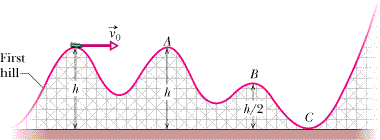
\includegraphics[scale=1]{hw8_problem3}
			\caption{Illustration of Problem 3}
			\label{fig:hw8_problem3}
		\end{center}
	\end{figure}

	\subsection{Question (a)}

		What is the speed of the car at point $A$?

		\textbf{R:}

		\begin{align}
			E_{tot,0} = \ &K_{0} + U_{g_{0}}& \notag \\
			= \ &\frac{1}{2} mv_{0}^{2} + mgy_{0}& \notag \\
			= \ &\left[\frac{1}{2}(16 \ sl)(16 \ ft/s)^{2}\right] + \left[(16 \ sl)\left(32.2 \ ft/s^{2}\right)(36 \ ft)\right]& \notag \\
			= \ &(2048 \ ft \times lb) + (18 \ 547.2 \ ft \times lb)& \notag \\
			= \ &20 \ 595.2 \ ft \times lb& \notag
		\end{align}

		\begin{align}
			E_{tot,1} = \ &K_{1} + U_{g_{1}}& \notag \\
			E_{tot,1} = \ &\frac{1}{2} mv_{1}^{2} + mgy_{1}& \notag \\
			v_{1} = \ &\sqrt{\frac{E_{tot,1} - mgy_{1}}{\frac{1}{2}m}}& \notag \\
			= \ &\sqrt{\frac{(20 \ 595.2 \ ft \times lb) - (18 \ 547.2 \ ft \times lb)}{8 \ sl}}& \notag \\
			= \ &\sqrt{\frac{2048 \ ft \times lb}{8 \ sl}}& \notag \\
			= \ &\sqrt{256 ft^{2}/s^{2}}& \notag \\
			= \ &16 \ ft/s&
		\end{align}

	\subsection{Question (b)}

		What is the speed of the car at point $B$?

		\textbf{R:}

		\begin{align}
			E_{tot,2} = \ &K_{2} + U_{g_{2}}& \notag \\
			E_{tot,2} = \ &\frac{1}{2} mv_{2}^{2} + mgy_{2}& \notag \\
			v_{2} = \ &\sqrt{\frac{E_{tot,2} - mgy_{2}}{\frac{1}{2}m}}& \notag \\
			= \ &\sqrt{\frac{(20 \ 595.2 \ ft \times lb) - (9273.6 \ ft \times lb)}{8 \ sl}}& \notag \\
			= \ &\sqrt{\frac{11 \ 321.6 \ ft \times lb}{8 \ sl}}& \notag \\
			= \ &\sqrt{1415.2 ft^{2}/s^{2}}& \notag \\
			= \ &37.62 \ ft/s&
		\end{align}

	\subsection{Question (c)}

		What is the speed of the car at point $C$?

		\textbf{R:}

		\begin{align}
			E_{tot,3} = \ &K_{3} + U_{g_{3}}& \notag \\
			E_{tot,3} = \ &\frac{1}{2} mv_{3}^{2} + mg(0)& \notag \\
			v_{3} = \ &\sqrt{\frac{E_{tot,3}}{\frac{1}{2}m}}& \notag \\
			= \ &\sqrt{\frac{20 \ 595.2 \ ft \times lb}{8 \ sl}}& \notag \\
			= \ &\sqrt{2574.4 ft^{2}/s^{2}}& \notag \\
			= \ &50.74 \ ft/s&
		\end{align}

	\subsection{Question (d)}

		How high will the car go on the last hill, which is too high for it to cross?

		\textbf{R:}

		\begin{align}
			E_{tot,4} = \ &K_{4} + U_{g_{4}}& \notag \\
			E_{tot,4} = \ &\frac{1}{2} m(0)^{2} + mgy_{4}& \notag \\
			y_{4} = \ &\frac{E_{tot,4}}{mg}& \notag \\
			= \ &\frac{20 \ 595.2 \ ft \times lb}{(16 \ sl)\left(32.2 \ ft/s^{2}\right)}& \notag \\
			= \ &\frac{20 \ 595.2 \ ft \times lb}{515.2 \ lb}& \notag \\
			= \ &39.98 \ ft&
		\end{align}
